\chapter{Representation changes through learning}
% \begin{figure}
%     \centering
%     \begin{tabular}{c}
% \includegraphics[width=14cm]{elementos-textuais/PFC_init_vs_end_heatmap.eps}
%     \\
% \includegraphics[width=14cm]{elementos-textuais/STR_PFC_day1_vs_day2.eps}
%     \end{tabular}
%     \caption[Representation changes with learning]{Representation changes with learning. The images show  \textbf{top:} The diagonal gets a little less clear in the second half of the session. \textbf{bottom:} Both PFC at day 2 and STR at day 1 have no detectable diagonal.} 
%     \label{fig:str_vs_pfc}
% \end{figure}

\begin{figure}
    \centering
    \begin{tabular}{cc}

    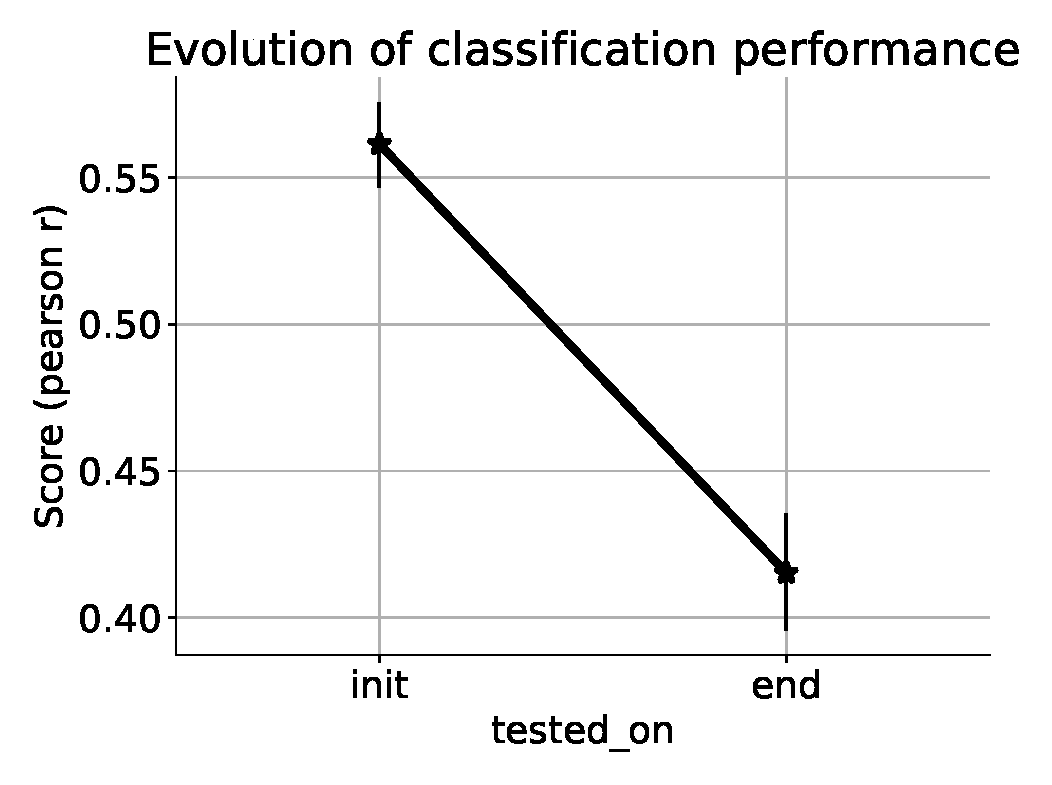
\includegraphics[width=7cm]{figures/PFC_init_vs_end.eps}
    & 
    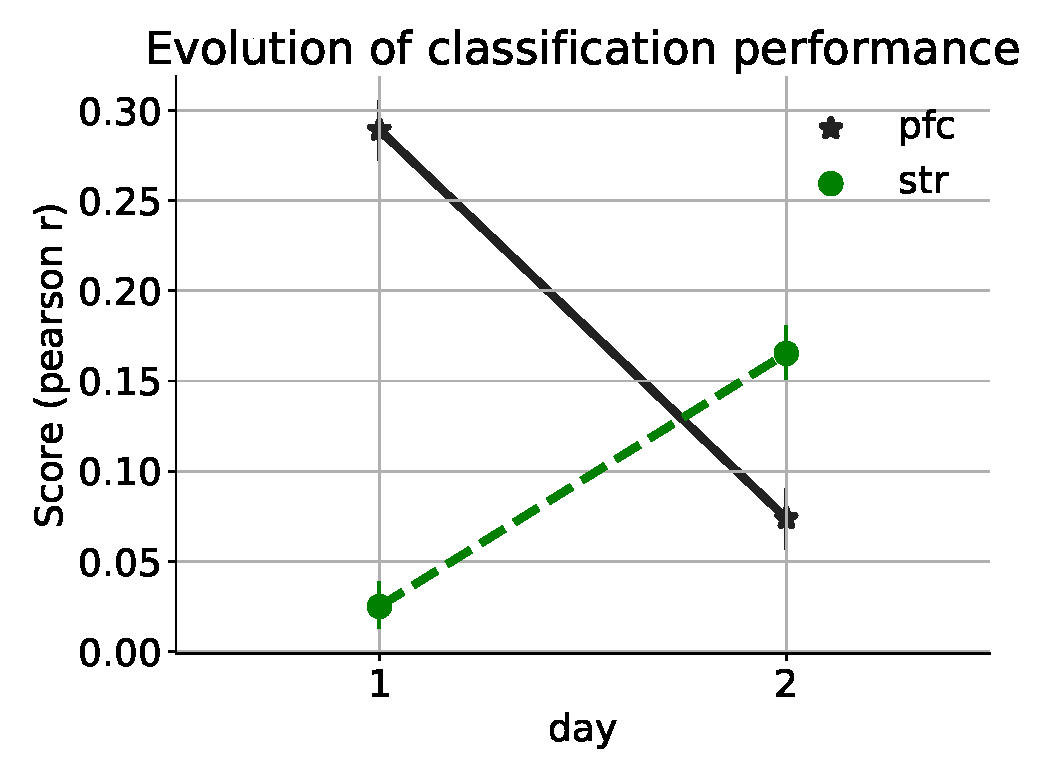
\includegraphics[width=7cm]{figures/STR_PFC_day1_vs_day2_evo.eps}
    \end{tabular}
    
    \caption[Striatum representation enhancement follows PFC's deterioration]{Striatum representation enhancement follows PFC's deterioration. Left: Group 1 at first vs second half of session. Right: Group 2, in different days.}
    \label{fig:clf_decrease}
\end{figure}

We want to measure how the time representation changes during learning, and the classification analysis just presented provided us with a validated classifier and dataset that allow us to tackle this question. Now we assess the resolution of time representation in the beginning of the animals' training, comparing it to when the animal is performing better. As discussed, we use classifier's performance as a proxy for time representation. For one set of animals we had long sessions of more than 1000 trials $(1149 \pm 384)$ with sufficient correct trials $(660 \pm 260)$, and in this case we split correct trials into first and second half. For the second set of animals, in which sessions were half as long with $570 \pm 181$ trials and $284\pm 100$ correct ones, we instead compared correct trials in the first versus second session. 

We can see in figure \ref{fig:str_vs_pfc} that the probability matrix is not random, and it has the highest values at the top left and lower right corners. This corners are mostly in the diagonal, which means classification is better at the borders, what may be due to the fact that classification in the borders is less ambiguous, since time bins at the borders have only half as many neighbour bins. In some cases the presence of a diagonal is clear, indicating that time points are in fact distinguishable by the classifier. In the STR/PFC images it is possible to perceive a stronger diagonal and weaker off-diagonal in the PFC's day 1 and STR's day 2, in comparison with the same area in the other day. This indicates that these areas do change through learning. The fact that the changes are opposite between areas indicates that their direction of change is inversely proportional.

When we look instead to final scores of classification performance, measured by Pearson's correlation, we can see that the changes in mPFC are consistent across datasets:  mPFC's time representation gets weaker as the session proceeds. Although this decrease was not clear in figure \ref{fig:str_vs_pfc}, in figure \ref{fig:clf_decrease} the decrease in performance can be seen inside a single session. Furthermore, in the comparison of two sessions, the performance agrees with the previous image, being higher where the diagonal is stronger. While it is clear that PFC's representation of time indeed weakens, the striatum later develops a representation that was not present in the first session. This result sheds some light in our unexpected finding that mPFC's time representation was decreasing with learning, suggesting that the role of representing time for this task may change dependencies through learning.

%Although we already removed the end of the session, when the animal is clearly not engaged, comparing between two sessions increases reliability in this aspect.
% In the right panel, we compared the neural representation of time in the PFC and Striatum in the first versus second session. In this entirely different dataset, The effect on the PFC agreed with the previous, in which classifier performance decreases in the prefrontal cortex after learning.

% Explicar mais profundamente, devagar e sem pressa
% \subsection{Baseline analysis}
% To better understand the role of the mPFC in our current task, we stored the neural activity not only inside the trials, but also in the 500ms prior to the animal entering the nosepoke, to understand if there were already activity predictive of the animal's responses, which could be interpreted as their current goal \cite{miller2001integrative} or, following the literature, as their internal representation of the task being performed \cite{durstewitz2010abrupt}. 

% Because there is difference in many neurons \change{difference in what??}, such as those in figure \ref{fig:Dcohen}'s lower pannels, it seems that before entering the nosepoke the animal already has some tendency either to leave it earlier than needed, or to hold longer. This difference has been assessed by Cohen's D measure of effect size, and many neurons have these differences in baseline activity.

% \begin{figure}
%     \centering
%     \includegraphics[width=\textwidth]{figuras/methods/two_cohenD.png}
%     \caption[Activity in the baseline predicts behavior]{Activity in the baseline predicts behavior. At the top, the measure of Cohen's D for each neuron, at the point of maximum difference in the baseline. At botton, an example neuron with different activity, with 95\% confidence interval around the mean.}
%     \label{fig:Dcohen}
% \end{figure}